\chapter{Introducción a la Programación Concurrente}
\section{Conceptos básicos}
Hasta ahora, nos hemos dedicado al estudio y desarrollo de programas secuenciales, que podemos entender de forma intuitiva como una ejecución lineal de instrucciones.\\

En programación concurrente, tendremos ahora múltiples unidades de ejecución independientes, a las que llamaremos procesos (sea un core o un procesador). La programación concurrente trata de coordinar los procesos para que cooperen entre sí con el fin de realizar un problema global de forma mucho más rápida de como lo haría un programa secuencial.\\

Podemos pensar que un proceso es una unidad de software abstracta conformada por con un conjunto de instrucciones a ejecutar y por el contexto del procesador (como los valores de los registros, el contador de programa, el puntero de pila, la memoria Heap, memoria para variables, el acceso a determinados recursos, \ldots), al que llamamos estado del proceso.\\

Cuando en esta asignatura aparezca ``flujo de control'', debemos pensar en una secuencia de ejecución de instrucciones. Es decir, como si fuera un proceso pero carante de un estado.\\

Nuestro trabajo en esta asignatura será gestionar la concurrencia, es decir, la ejecución independiente de dichos procesos con el fin de que no sea una sucesión de eventos incontrolados.

% // TODO: Cambiar este titulo
\subsection{Comparación de programas concurrentes con secuenciales}
Normalmente, en un programa concurrente tendremos más procesos que núcleos donde ejecutar dichos procesos, de donde aparece el concepto de concurrencia: en programación concurrente debe parecer que todos los procesos avanzan de forma simultánea, pese a haber más procesos que núcleos.\\

Si provocamos cambios de contexto dejando avanzar al resto de flujos de control, el programa no sufrirá las latencias provocadas por los procesos de E/S (por ejemplo), haciendo que el programa global sea más eficiente gracias a la concurrencia.\\

En sistemas que simulen el mundo real, podemos asociar un proceso con cada ente que intervenga en nuestro sistema (como una simulación del tráfico en una ciudad, o del movimiento de planetas), con lo que los sistemas de simulación pueden modelarse mejor con procesos concurrentes independientes, más que con programas secuenciales.

\subsection{Definición de concurrencia}
Podríamos definir la concurrencia como el paralelismo potencial que existe en los programa que puede aprovecharse independientemente de las limitaciones del hardware en el que se ejecuta el programa.\\

Como ya hemos mencionado, podremos tener un mayor número de procesos que de cores, y con este modelo cada uno de los procesos se ejecuta aparentemente al mismo tiempo que los demás.\\

El concepto de concurrencia es un concepto de programación a alto nivel que trata de representar el paralelismo potencial que existe en un programa. Con los compiladores adecuados, podemos programar en función de dichas características sin limitarnos por la arquitectura hardware del ordenador.\\

El objetivo fundamental de la concurrencia es simplificar toda la parte de la sincronización y comunicación entre los diferentes procesos de un programa, el cual suele ser un problema complejo sin solución fácil. Nos da un nivel algorítmico suficientemente independiente de los detalles del hardware para resolver dichos problemas, facilitando la portabilidad del código entre arquitecturas y lenguajes de programación.\\

\noindent
Como beneficios de este modelo abstracto (el de la concurrencia), podemos destacar:
\begin{itemize}
    \item Da herramientas, instrucciones y sentencias útiles para problemas de sincronización entre procesos.
    \item Las primitivas de programación en un lenguaje de alto nivel (como son los lenguajes concurrentes) son más fáciles de utilizar que con lenguajes de bajo nivel. Por ejemplo, los semáforos son más complejos que los monitores.
    \item Evita la dependencia con instrucciones de bajo nivel, haciendo que el programa pueda ejecutarse en otra computadora.
\end{itemize}

\subsection{Axiomas de la programación concurrente}
La programación concurrente es un modelo abstracto definido en base a 5 axiomas que nos dicen si un lenguaje es o no concurrente. En caso de no cumplirse, el código no va a poder ser transportable ni verificable.

Estos axiomas son:
\begin{description}
    \item [1. Atomicidad y entrelazamiento de instrucciones atómicas.]~\\
        Al menos ciertas instrucciones han de ser atómicas (esto es, instrucciones que no pueden ser interrumpidas, como por ejemplo las lecturas y escrituras en memoria).
    \item [2. Consistencia de los datos tras un acceso concurrente.]~\\
        Si tenemos muchos procesos actuando a la vez sobre un conjunto de datos compartidos, debemos estar seguros de que los accesos a los mismos no los estropeen.
    \item [3. Irrepetibilidad de las secuencias de instrucciones.]~\\
        Cuando se ejecuta un programa concurrente, se sucede un entrelazamiento de las instrucciones de los procesos que se ejecutan a la vez, con lo que la secuencia de instrucciones que obtenemos como resultado de volver a ejecutar el mismo programa con otros datos es muy probable que no sea la misma.

        Esto dificulta el debugging de un programa concurrente, ya que podemos tener un error en el programa que repercuta en el mal funcionamiento del mismo sólo cuando se suceda una secuencia de instrucciones específica en la ejecución del mismo.
    \item [4. Independencia de la velocidad de los procesos.]~\\
        No puede hacerse ninguna suposición en la velocidad de ejecución de un proceso, ya que este puede verse suspendido o ralentizado.

        La corrección en programas concurrentes no debe depender de la velocidad relativa de los procesos.
    \item [5. Hipótesis del progreso finito.]~\\
        \begin{itemize}
            \item Un proceso debe tratar de avanzar todo lo que pueda. Esto es, si un proceso se está ejecutando, debe tratar de ejecutar tantas instrucciones como sea posible.
            \item Una vez que un proceso comienza a ejecutar una sección de código, debe terminar dicha sección.
            \item Todo proceso debe seguir progresando durante la ejecución de un programa.
        \end{itemize}
\end{description}

\noindent
Cuando se interpreta la ejecución de un programa concurrente como un conjunto de trazas de las cuales elegimos una al ejecutar el programa, estamos ignorando ciertos detalles, como:
\begin{itemize}
    \item El estado de la memoria asignado a cada proceso.
    \item El valor de los registros de cada proceso.
    \item El coste computaciones de los cambios de contexto.
    \item La política de planificación que se emplea de los procesos.
    \item El desarrollo de los programas es independiente del hardware.
\end{itemize}

\section{Modelos para creación de procesos en un programa}
En relación al número de procesos que se ejecutan en un programa, podemos clasificarlos en:
\begin{itemize}
    \item Sistemas estáticos: El número de proesos en el programa es el mismo durante su ejecución. Dicho número se define al programarlo y en el momento de la compilación.
    \item Sistemas dinámicos: El número de procesos es variable, de forma que durante la ejecución del programa pueden crearse y destruirse procesos.
\end{itemize}

\subsection{Grafos de Sincronización}
Un Grafo de Sincronización es un Grafo Dirigido Acíclico (DAG) donde cada nodo representa una secuencia de sentencias del programa (o actividad). Nos sirven para definir situaciones de preferencia en la ejecución de un programa. Tenemos que tener instrucciones en el lenguaje concurrente que nos permitan representar el comienzo de las instrucciones con un DAG\@.\\

En un DAG, se succeden dependencias secuenciales, esto es, un proceso no empieza hasta que termina otro: dadas dos actividades $S_1$ y $S_2$, una arista desde la primera hacia la segunda ($S_1\rightarrow S_2$) significa que $S_2$ no puede comenzar su ejecución hasta que $S_1$ haya finalizado.\\

\begin{ejemplo}
    El DAG de la Figura~\ref{fig:primer_dag} nos indica que la primera actividad que tendrá lugar en nuestro programa será la actividad $S_1$. Tras el fin de esta, se sucederán de forma concurrente las actividades $S_2$ y $S_3$. Tras terminar $S_2$, comenzará $S_4$ y, tras esta, se ejecutarán de forma concurrente $S_5$ y $S_6$. Finalmente, tras el final de $S_5$, $S_6$ y $S_3$, el programa terminará con la actividad $S_7$.

    \begin{figure}[H]
    \centering
    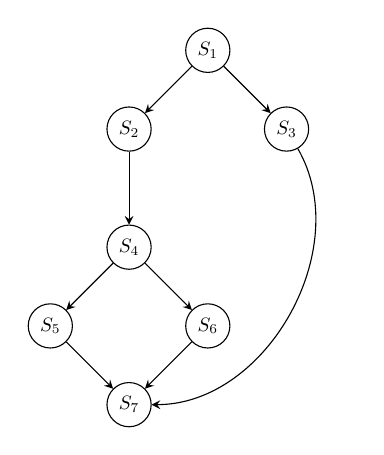
\begin{tikzpicture}
        \node[draw, circle, scale=0.7] (A) at (0,0) {$S_1$};
        \node[draw, circle, scale=0.7] (B) at (-1,-1) {$S_2$};
        \node[draw, circle, scale=0.7] (C) at (1,-1) {$S_3$};
        \node[draw, circle, scale=0.7] (D) at (-1,-2.5) {$S_4$};
        \node[draw, circle, scale=0.7] (E) at (-2,-3.5) {$S_5$};
        \node[draw, circle, scale=0.7] (F) at (0,-3.5) {$S_6$};
        \node[draw, circle, scale=0.7] (G) at (-1,-4.5) {$S_7$};
        
        \draw[-stealth] (A) -- (B);
        \draw[-stealth] (A) -- (C);
        \draw[-stealth] (B) -- (D);
        \draw[-stealth] (D) -- (E);
        \draw[-stealth] (D) -- (F);
        \draw[-stealth] (E) -- (G);
        \draw[-stealth] (F) -- (G);

        \draw[-stealth] (C) to[out=300, in=0] (G);
    \end{tikzpicture}
    \caption{Ejemplo de DAG}
    \label{fig:primer_dag}
    \end{figure}
\end{ejemplo}

\noindent
En relación a cómo podemos crear los procesos, destacamos dos formas que podemos encontrarnos en los lenguajes paralelos:

\subsection{Definición estructurada de procesos}
En programación estructurada, contaremos con dos palabras reservadas del lenguaje que nos permitirán recrear la siguiente funcionalidad a explicar. En pseudocódigo, nos referiremos a ellas como \verb|cobegin| y \verb|coend|.\\

Dados dos procesos $P_1$ y $P_2$ que queremos que se ejecuten de forma concurrente, bastará especificar en pseudocódigo:
\begin{minted}{pascal}
    cobegin
      P1; 
      P2; 
    coend
\end{minted}
Hasta llegar a la palabra \verb|cobegin| no comenzará ningún proceso. Tras esta, se sucederá un entrelazado de las instrucciones de $P_1$ y $P_2$, y no se saldrá de dicha región hasta que terminen ambos procesos.

\begin{ejemplo}
    Un programa utilizando la definición estructurada de procesos que cumpla el DAG de la Figura~\ref{fig:primer_dag} es el siguiente:
    \begin{minted}{pascal}
    begin
      S1;
      cobegin
        begin
          S2;
          S4;
          cobegin
            S5;
            S6;
          coend
        end
        S3;
      coend
      S7;
    end
    \end{minted}
\end{ejemplo}

\subsection{Definición no estructurada de procesos}
En lenguajes concurrentes que no cuenten con palabras reservadas que simulen \verb|cobegin| y \verb|coend|, contaremos con dos llamadas al sistema que nos permitirán replicar dicha funcionalidad para crear procesos:
\begin{description}
    \item [fork]~\\
        Duplica el proceso que actualmente se está ejecutando y lo lanza a ejecución. Si se el especifica una rutina, cambiará el código del clon por dicha rutina.
    \item [join]~\\
        Espera a que cierto proceso termine de ejecutarse antes de proseguir con la ejecución del resto de instrucciones.
\end{description}
La función \verb|fork| ya se vió en la asignatura de Sistemas Operativos, por lo que el estudiante debería estar familiarizado con ella.

\begin{ejemplo}
    Un programa con definición no estructurada de procesos para el DAG de la Figura~\ref{fig:primer_dag} es el siguiente:
    \begin{minted}{pascal}
    begin        
      S1;
      fork S3;
      S2;
      S4;
      fork S6;
      S5;
      join S3;
      join S6;
      S7;
    end
    \end{minted}
\end{ejemplo}

\section{Exclusión mutua y sincronización}
No todas las secuencias de entrelazamiento de un programa concurrente van a ser aceptables. Para impedir que sucedan ciertas secuencias (o trazas) tenemos condiciones de sincronización, relacionadas con instrucciones de lenguajes de programación de tal forma que dichas instrucciones no se ejecutan hasta que no es cierta una condición que depende de las variables del proceso.

De esta forma, una \textbf{condición de sincronización} es una restricción en el orden en que se pueden entremezclar las instrucciones que generan los procesos de un programa. Podemos utilizarlas para asegurarnos de que todas las trazas del programa son correctas.\\

La \textbf{exclusión mutua} es un caso particular de sincronización en el que se obliga a que un trozo de código de un proceso sea ejecutado de forma totalmente secuencial de manera que no se permita el entrelazamiento con otros procesos. Este trozo de código (en el que no se permite el entrelazamiento de instrucciones con otros procesos) recibe el nombre de \textbf{sección crítica}. Se dice que las secciones críticas se ejecutan en exclusión mutua.\\

La mayoría de instrucciones en un programa son instrucciones compuestas (esto es, formadas por varias instrucciones en lenguaje máquina). Si queremos establecer secciones críticas para la ejecución de cada una de dichas instrucciones, rodearemos la instrucción por \verb|<| y \verb|>|.

\begin{ejemplo}
    Por ejemplo, ante el siguiente código concurrente:
    \begin{minted}{pascal}
    begin
      x := 0;
      cobegin
        x := x+1;
        x := x-1;
      coend
    end
    \end{minted}
    El resultado obtenido en la variable \verb|x| es indeterminado, ya que puede ser 1, -1 o 0:
    \begin{itemize}
        \item El segundo proceso puede leer la variable \verb|x| antes de que el primero escriba en ella, leyendo 0; y podría escribir en ella después de que lo haga el primer proceso, escribiendo finalmente un -1.
        \item Podría ejecutarse el primer proceso antes que el segundo, dejando la variable \verb|x| a 1 y el segundo le cambiaría el valor a 0.
        \item El primer proceso puede leer la variable \verb|x| antes de que el segundo escriba en ella, leyendo 0; y podría escribir en ella después de que lo haga el segundo proceso, escribiendo finalmente un 1.
    \end{itemize}
    Notemos que esto sucede ya que la instrucción \verb|x := x OP a| es una instrucción compuesta de las instrucciones máquina: \verb|LOAD x|, \verb|OP a, x| y \verb|STORE x|.

    Sin embargo, ante el siguiente código concurrente:
    \begin{minted}{pascal}
    begin
      x := 0;
      cobegin
        < x := x+1 >;
        < x := x-1 >;
      coend
    end
    \end{minted}
    Obtenemos siempre 0 en \verb|x|, ya que las instrucciones de cada instrucción compeusta no se entrelazan, al ser secciones críticas. 
\end{ejemplo}

\subsubsection{Paradigma del Productor Consumidor}
El paradigma del productor/consumidor es una situación de dos procesos que cooperan, uno escribiendo datos en una variable, al que llamaremos productor; y otro que leerá dicha variable y realizará cálculos con ella, al que llamaremos consumidor.

Este paradigma nos sirve de ejemplo para justificar las condiciones de sincronización, así como para ponerlas en práctica.\\

Son necesarias condiciones de sincronización ya que no todas las trazas de ejecución de un programa con estructura productor/consumidor son correctas.

\begin{ejemplo}
    Si notamos por $L$ a las lecturas del consumidor y por $E$ a las escrituras del productor, las tres siguientes trazas de ejecución no son correctas:
    \begin{enumerate}
        \item \verb|L, E, L, E, ...|, porque leemos una lectura de la variable antes de que el productor escriba en ella, leyendo un valor indeterminado y puediendo provocar el fallo del programa.
        \item \verb|E, L, E, E, L, ...|, porque el consumidor se ha perdido una escritura del productor en la variable, que puede hacer que cambie la salida del programa a una errónea.
        \item \verb|E, L, L, E, L, ...|, porque el consumidor ha usado un mismo dato dos veces, que también puede resultar en un mal funcionamiento del programa.
    \end{enumerate}
\end{ejemplo}

Para que el paradigma del productor/consumidor funcione correctamente, han de cumplirse las dos condiciones de sincronización siguientes:
\begin{enumerate}
    \item El consumidor no puede leer la variable hasta que el productor no haya escrito en ella. Cuando el consumidor lee, debe esperar a que el productor proporcione un nuevo dato antes de volver a leer.
    \item El productor no puede escribir un nuevo valor hasta que el consumidor haya leido el último dato escrito (salvo en el primer valor a escribir).
\end{enumerate}
Para cumplir con las condiciones de sincronización, deberemos añadir instrucciones en el código para que:
\begin{itemize}
    \item El consumidor se detenga la primera vez hasta que el productor escriba en la variable.
    \item Se impida un segundo ciclo del consumidor hasta que se produzca el siguiente dato.
    \item Se impida un segundo ciclo del productor hasta que el dato anterior no haya sido leído por el consumidor.
\end{itemize}

\section{Corrección en los programas concurrentes}
En los programas secuenciales, para comprobar la corrección de los mismos, debemos probar que el programa termina dando salidas previstas ante determinadas entradas.

En un programa secuencial, hay un único conjunto de datos de entrada que provoca un único conjunto de datos de salida. Esto no sucede en programas concurrentes, ya que el indeterminismo en la ejecución provoca distintas trazas posibles del programa, y es bastante probable que todas las trazas posibles no provoquen los mismos resultados.\\

Para comprobar que un programa concurrente es correcto o no, podemos decir que lo es o no en función de los requisitos del programa requeridos.

Por ejemplo, dada la especificación del paradigma del productor/consumidor, decimos que un programa que lo implemente es correcto si en todas sus ejecuciones garantiza una traza que se corresponde con \verb|L, E, L, E,| \ldots. Probar esto es algo difícil todavía.

\subsection{Propiedades de los programas concurrentes}
Observando el software concurrente, hay dos tipos de especificaciones que son estáticas y están perfectamente definidas durante la ejecución del programa; que pueden definirse en el momento de la compilación.

\subsubsection{Propiedades de seguridad}
Son condiciones que deben cumplirse en cada instante de la traza de un programa.

